\documentclass[11pt,a4paper]{article}

\usepackage{kotex}
\usepackage{amsmath,amssymb,amsthm,mathtools,bm}
\usepackage{booktabs,tabularx,longtable,array}
\usepackage{graphicx}
\usepackage{caption}
\usepackage{subcaption}
\usepackage{geometry}
\usepackage{enumitem}
\usepackage{xcolor}
\usepackage{hyperref}
\usepackage{listings}
\usepackage{float}
\usepackage{tcolorbox}
\tcbuselibrary{breakable,skins}

\geometry{margin=25mm}
\graphicspath{{report_figures/}}
\hypersetup{
  colorlinks=true,
  linkcolor=blue!60!black,
  citecolor=blue!60!black,
  urlcolor=blue!60!black
}
\setlist[itemize]{leftmargin=2em}
\setlist[enumerate]{leftmargin=2em}
\lstset{
  basicstyle=\ttfamily\small,
  breaklines=true,
  frame=single,
  columns=fullflexible
}
\sloppy

% ---- 수학 매크로 ----
\newcommand{\E}{\mathcal{E}}
\newcommand{\N}{\mathcal{N}}
\newcommand{\Hcal}{\mathcal{H}}
\newcommand{\Tr}{\operatorname{Tr}}
\newcommand{\Choi}{C_{\mathcal{E}}}
\newcommand{\id}{\mathrm{id}}
\newcommand{\Pos}{\mathrm{Pos}}
\newcommand{\Dens}{\mathrm{D}}
\newcommand{\Lin}{\mathrm{L}}
\newcommand{\diamondnorm}[1]{\left\lVert #1 \right\rVert_{\diamond}}
\newcommand{\onenorm}[1]{\left\lVert #1 \right\rVert_{1}}
\newcommand{\rank}{\operatorname{rank}}
\newcommand{\vecop}{\operatorname{vec}}
\DeclareMathOperator{\sgn}{sgn}

% ---- 정리 환경 ----
\theoremstyle{definition}
\newtheorem{definition}{정의}[section]
\newtheorem{example}{예제}[section]
\theoremstyle{plain}
\newtheorem{theorem}{정리}[section]
\newtheorem{proposition}{명제}[section]
\newtheorem{property}{성질}[section]
\newtheorem{corollary}{따름정리}[section]
\theoremstyle{remark}
\newtheorem*{remark}{참고}

% ---- 색상 상자 ----
\newtcolorbox{conceptbox}[1]{
  colback=blue!4!white, colframe=blue!50!black,
  fonttitle=\bfseries, title={#1},
  breakable, boxrule=0.6pt, arc=2pt}
\newtcolorbox{intuitionbox}{
  colback=green!4!white, colframe=green!45!black,
  breakable, boxrule=0.6pt, arc=2pt,
  left=4pt,right=4pt,top=3pt,bottom=3pt}
\newtcolorbox{mathbox}[1]{
  colback=orange!4!white, colframe=orange!55!black,
  fonttitle=\bfseries, title={#1},
  breakable, boxrule=0.6pt, arc=2pt}

\title{\textbf{양자 채널의 Choi 표현을 이용한 채널 분석과 응용\\[5pt]
\large{--- 직관과 수식을 함께 담은 통합 개정본 (REVISED) ---}}}
\author{Choi Representation Multi-Agent Project}
\date{\today}

\begin{document}
\maketitle

\begin{abstract}
이 개정본은 같은 프로젝트의 두 판본 --- 직관 중심의 ``초심자용 안내서''와 수식 중심의 ``이론 해설본'' --- 을 \textbf{하나로 통합}하고, 이해를 돕는 내용(읽기 경로, 손계산 예제, 요약 치트시트, 용어집)을 보강한 것이다. 목표는 ``양자 채널을 \textbf{Choi 행렬}이라는 하나의 행렬로 바꾸면, 서로 달라 보이는 다섯 가지 주제가 모두 같은 언어로 연결된다''는 주장을, \emph{왜 그런지에 대한 직관}과 \emph{검증 가능한 등식·정리}로 동시에 제시하는 것이다.

이를 위해 본문은 모든 핵심 개념을 (i)~말로 된 \emph{직관}, (ii)~번호 붙은 \emph{정의/성질/정리}, (iii)~한 줄 \emph{수식 요약}의 세 겹으로 설명한다. 양자역학의 가장 기초(상태, 측정, 중첩)만 아는 독자를 위해 밀도행렬·텐서곱·부분 대각합·양자 채널·완전양성성(CP)·대각합 보존(TP)·Bloch 구를 먼저 엄밀히 정의한 뒤, 채널의 세 동치 표현(Kraus, Stinespring, Choi)과 이들을 잇는 \textbf{Choi--Jamio{\l}kowski 동형사상}
\[
\E\text{ CP}\iff C_\E\succeq0,\qquad \E\text{ TP}\iff \Tr_B(C_\E)=I_A
\]
을 증명 개요와 함께 제시한다. 그 위에서 다섯 작업---표현 변환 검증, process tomography, diamond norm 기반 channel discrimination, quantum comb를 이용한 non-Markovian 분석, interactive 시각화---을 각각 fidelity 관계식 $F_{\mathrm{avg}}=\frac{dF_{\mathrm{pro}}+1}{d+1}$, Helstrom 한계, Watrous SDP, BLP/RHP measure, link product 같은 정량적 도구와 함께 전개한다. 모든 그림·표·수치는 원본과 동일하게 유지하되, 각 수치가 \emph{어떤 식에서 나오는지}를 명시한다.
\end{abstract}

\tableofcontents
\newpage

%==================================================================
\section{이 보고서를 읽는 방법}
%==================================================================

이 개정본은 한 권 안에서 \textbf{직관과 수식을 모두} 제공한다. 따라서 독자의 배경에 따라 두 가지 읽기 경로를 권한다.

\begin{itemize}
  \item \textbf{직관 트랙(처음 접하는 독자):} 각 절의 파란 \emph{개념 상자}와 초록 \emph{직관 요약}을 먼저 따라 읽고, 정리와 증명은 건너뛴다. 그림과 표의 해석 문단을 읽으면 큰 줄기를 잡을 수 있다.
  \item \textbf{수식 트랙(이론을 확인하려는 독자):} 번호 붙은 \emph{정의/성질/정리}와 주황 \emph{수식 상자}를 중심으로 읽는다. 각 수치 결과에는 그것을 낳는 식이나 정리 번호가 달려 있다.
\end{itemize}

\begin{conceptbox}{세 가지 상자의 역할}
\begin{description}[leftmargin=1.4em,style=nextline]
  \item[\textcolor{blue!60!black}{$\blacksquare$} 개념 상자 (파랑)] 새 용어를 도입하고 그 의미를 설명한다.
  \item[\textcolor{green!50!black}{$\blacksquare$} 직관 요약 (초록)] ``결국 한 문장으로 무슨 뜻인가''를 정리한다.
  \item[\textcolor{orange!70!black}{$\blacksquare$} 수식 상자 (주황)] 정의식·핵심 성질·수치 재현을 모은다.
\end{description}
또한 \emph{정의 / 성질 / 명제 / 정리 / 예제}는 번호가 붙은 환경으로 제시하여 추적이 가능하다.
\end{conceptbox}

\begin{conceptbox}{표기 약속(notation)}
\begin{itemize}[leftmargin=1.4em]
  \item $\Hcal_A,\Hcal_B$: 유한 차원 복소 Hilbert 공간, $d_A=\dim\Hcal_A$. 큐비트는 $d=2$.
  \item $\Lin(\Hcal)$: $\Hcal$ 위 선형연산자 전체. $\Pos(\Hcal)=\{X\succeq0\}$, $\Dens(\Hcal)=\{\rho\succeq0,\Tr\rho=1\}$.
  \item $X^\dagger$ 켤레전치, $X^T$ 전치, $\overline{X}$ 성분별 켤레복소.
  \item $\succeq0$: 양의 준정부호(모든 고유값 $\ge0$). $\onenorm{X}=\Tr\sqrt{X^\dagger X}$: 대각합 노름.
  \item $I_A$ 항등연산자, $\{|i\rangle\}$ 계산기저, 파울리 $X,Y,Z$, $\vec\sigma=(X,Y,Z)$.
\end{itemize}
\end{conceptbox}

마지막에 \textbf{부록 A}로 ``개념 $\to$ 직관 $\to$ 핵심 식''을 한 장에 모은 요약 치트시트와, \textbf{부록 B}로 영문 용어집을 두었다. 급할 때는 부록 A만 보아도 전체 지도를 얻을 수 있다.

%==================================================================
\section{준비: 본론을 읽기 위한 도구들}
%==================================================================

이 장의 목표는 하나다. 3장에서 ``채널을 Choi 행렬로 바꾼다''는 문장이 나왔을 때, 그 한 문장의 모든 단어가 이미 친숙해지도록 만드는 것이다. 각 도구를 직관과 수식으로 동시에 정의한다.

\subsection{양자 상태: 상태벡터에서 밀도행렬로}

기초 양자역학에서 한 양자계의 상태는 상태벡터 $|\psi\rangle$로 적는다. 큐비트는 $|\psi\rangle=\alpha|0\rangle+\beta|1\rangle$, $|\alpha|^2+|\beta|^2=1$처럼 두 기저 상태의 중첩이다. 이렇게 단 하나의 벡터로 완전히 적히는 상태를 \textbf{순수 상태}라 한다. 그러나 실제로는 ``70\%로 $|0\rangle$, 30\%로 $|1\rangle$''처럼 \emph{고전적 확률이 섞인} \textbf{혼합 상태}가 흔하고, 이는 하나의 벡터로 적을 수 없다. 그래서 \textbf{밀도행렬} $\rho$를 도입한다.

\begin{conceptbox}{개념: 밀도행렬 $\rho$}
순수 상태는 $\rho=|\psi\rangle\langle\psi|$, 혼합 상태는 확률 $p_k$로 $\rho=\sum_k p_k|\psi_k\rangle\langle\psi_k|$. 직관적으로 ``상태에 대해 우리가 아는 모든 통계''를 담은 행렬이다.
\end{conceptbox}

\begin{definition}[밀도행렬]
계 $\Hcal$의 상태는 $\rho=\rho^\dagger,\ \rho\succeq0,\ \Tr\rho=1$을 만족하는 연산자 $\rho\in\Lin(\Hcal)$이다.
\end{definition}

\begin{property}[밀도행렬의 기본 성질]\label{prop:density}
임의의 밀도행렬 $\rho$에 대하여:
\begin{enumerate}[label=\textup{(\roman*)}]
  \item \textbf{스펙트럼 분해} $\rho=\sum_i\lambda_i|e_i\rangle\langle e_i|$, $\lambda_i\ge0,\ \sum_i\lambda_i=1$ (고유값들이 확률분포를 이룬다).
  \item \textbf{기댓값} $\langle A\rangle=\Tr(\rho A)$.
  \item \textbf{순도} $\Tr(\rho^2)=\sum_i\lambda_i^2\le1$, 등호 $\iff$ 순수 상태.
\end{enumerate}
\end{property}
\begin{proof}[증명 개요]
(i)~에르미트·$\succeq0$이므로 스펙트럼 정리로 $\lambda_i\ge0$, $\sum_i\lambda_i=\Tr\rho=1$. (ii)~$\Tr$의 선형성·순환성. (iii)~$\sum\lambda_i=1,\lambda_i\ge0\Rightarrow\sum\lambda_i^2\le(\sum\lambda_i)^2=1$, 등호는 rank-1.
\end{proof}

\begin{intuitionbox}
\textbf{직관:} 성질 \ref{prop:density}의 ``\emph{고유값이 음이 아니다}''와 정의의 ``\emph{대각합이 1이다}''라는 두 조건이 이 보고서 전체의 씨앗이다. 채널의 물리성 조건(CP/TP)이 바로 이 둘의 일반화다.
\end{intuitionbox}

\subsection{대각합과 부분 대각합}

\begin{conceptbox}{개념: 대각합·부분 대각합}
\textbf{대각합} $\Tr(M)$은 대각 성분의 합으로, $\Tr(\rho)$는 ``전체 확률'', $\Tr(\rho A)$는 ``$A$의 기댓값''. \textbf{부분 대각합}은 합동 상태에서 \emph{한 계를 측정하지 않고 무시}했을 때 남는 상태를 준다.
\end{conceptbox}

\begin{definition}[부분 대각합]
$\Tr_B:\Lin(\Hcal_A\otimes\Hcal_B)\to\Lin(\Hcal_A)$,
\[
\Tr_B(M)=\sum_k(I_A\otimes\langle k|_B)\,M\,(I_A\otimes|k\rangle_B),
\]
$\{|k\rangle_B\}$는 임의의 정규직교기저(정의는 기저 무관).
\end{definition}

\begin{property}[부분 대각합의 성질]\label{prop:ptrace}
$\Tr_B$는 선형이고 $\Tr_A\circ\Tr_B=\Tr$, $\Tr_B(\rho_A\otimes\rho_B)=\rho_A\Tr(\rho_B)$, 그리고 $M\succeq0\Rightarrow\Tr_B(M)\succeq0$. 환원 상태는 $\rho_A=\Tr_B(\rho_{AB})$.
\end{property}

\subsection{두 계를 합치기: 텐서곱과 얽힘}

큐비트 여럿을 함께 다루려면 \textbf{텐서곱} $\otimes$가 필요하다. 차원 $d_A,d_B$의 두 계를 합치면 합동계는 차원 $d_Ad_B$가 된다(큐비트 둘이면 $4$, 기저 $|00\rangle,|01\rangle,|10\rangle,|11\rangle$).

\begin{conceptbox}{개념: 얽힘(entanglement)}
합동 상태가 항상 $\rho_A\otimes\rho_B$처럼 두 부분의 곱으로 쪼개지지는 않는다. 쪼개지지 않는 상태가 \textbf{얽힌} 상태다. 뒤에서 ``보이지 않는 참조계와의 얽힘''이 완전양성성(CP)과 채널 구별 성능의 열쇠가 된다.
\end{conceptbox}

\begin{definition}[최대 얽힘 상태]
$\Hcal_A\cong\Hcal_B\cong\mathbb C^d$에서 비정규화 $|\Omega\rangle=\sum_{i=1}^d|i\rangle_A|i\rangle_B$ ($\langle\Omega|\Omega\rangle=d$), 정규화 $|\Phi\rangle=\tfrac1{\sqrt d}|\Omega\rangle$. 큐비트에서 $|\Phi\rangle=\tfrac1{\sqrt2}(|00\rangle+|11\rangle)$.
\end{definition}

\begin{property}[ricochet/전치 항등식]\label{prop:ricochet}
임의의 $M$에 대해 $(M\otimes I)|\Omega\rangle=(I\otimes M^T)|\Omega\rangle$.
\end{property}
\begin{proof}
$(M\otimes I)|\Omega\rangle=\sum_{ij}M_{ji}|j\rangle|i\rangle$, $(I\otimes M^T)|\Omega\rangle=\sum_{ij}M_{ij}|i\rangle|j\rangle$. 더미 지표 $i\leftrightarrow j$ 교환으로 두 식이 같다.
\end{proof}

성질 \ref{prop:ricochet}은 Choi 행렬에서 채널 작용을 복원하는 공식(정리 \ref{thm:recover})과 SDP 절의 ``얽힘이 정보를 더한다''는 사실을 떠받친다.

\subsection{양자 채널: unitary만으로 부족한 이유}

닫힌 계의 변화는 unitary $U$로 $\rho\mapsto U\rho U^\dagger$이다(잡음 없음, 이상적). 그러나 실제 장치에서는 큐비트가 환경과 상호작용해 에너지가 새는 \textbf{relaxation}, 위상이 흐트러지는 \textbf{dephasing}, 보정 오차가 함께 일어난다. 이런 ``열린 계''의 변화는 unitary 하나로 적을 수 없고, 더 일반적인 \textbf{양자 채널}이 필요하다.

\begin{conceptbox}{개념: 양자 채널 $\E$와 CP/TP}
양자 채널은 밀도행렬을 밀도행렬로 보내는 선형 사상이다. 물리적이려면 \textbf{TP}(전체 확률 보존)와 \textbf{CP}(보이지 않게 얽힌 친구까지 고려해도 결과가 정상)를 만족해야 한다.
\end{conceptbox}

\begin{definition}[양자 채널]
선형 $\E:\Lin(\Hcal_A)\to\Lin(\Hcal_B)$가 다음을 만족하면 채널(CPTP)이다.
\begin{itemize}[leftmargin=1.6em]
  \item \textbf{TP:} 모든 $X$에 대해 $\Tr[\E(X)]=\Tr[X]$.
  \item \textbf{CP:} 모든 $n$에 대해 $\E\otimes\id_n$이 양성 보존, 즉 $X\succeq0\Rightarrow(\E\otimes\id_n)(X)\succeq0$.
\end{itemize}
\end{definition}

\begin{mathbox}{왜 ``양성''이 아니라 ``완전양성''인가}
$n=1$ 양성만으로는 부족하다. 반례는 전치 사상 $T(\rho)=\rho^T$로, $T$는 양성이나 완전양성이 아니다:
\[
(T\otimes\id)(|\Phi\rangle\langle\Phi|)=\tfrac12\,\mathrm{SWAP}\quad\text{는 고유값 }-\tfrac12\text{ 을 가진다.}
\]
즉 남몰래 얽힌 참조계까지 고려하면 $T$는 비물리적이다. CP는 ``임의의 참조계 확장에서도 정당함''을 요구한다.
\end{mathbox}

\begin{intuitionbox}
\textbf{직관:} TP는 ``확률이 새지 않는다'', CP는 ``남몰래 얽힌 친구까지 고려해도 결과가 정상이다''. 물리적 채널 $=$ TP $+$ CP. 이 추상적 조건을 \emph{계산 가능}하게 만드는 것이 3장의 Choi 행렬이다.
\end{intuitionbox}

\subsection{한 큐비트를 보는 그림: Bloch 구}

\begin{conceptbox}{개념: Bloch 구}
큐비트 상태는 $\rho=\tfrac12(I+\vec r\cdot\vec\sigma)$, $\vec r=(r_x,r_y,r_z)$로 단위 구 위/안의 점이 된다. 표면($|\vec r|=1$)은 순수, 내부는 혼합, 중심($\vec r=0$)은 완전 무질서 상태 $I/2$. 채널은 구를 아핀 변환 $\vec r\mapsto M\vec r+\vec t$로 \emph{찌그러뜨리고($M$) 중심을 옮긴다($\vec t$)}.
\end{conceptbox}

\begin{property}[Bloch 구와 PSD]
$\rho=\tfrac12(I+\vec r\cdot\vec\sigma)$의 고유값은 $\tfrac{1\pm|\vec r|}{2}$이고, 순도는 $\Tr(\rho^2)=\tfrac{1+|\vec r|^2}{2}$. 따라서 $\rho\succeq0\iff|\vec r|\le1$.
\end{property}

\begin{conceptbox}{개념: unital 채널}
$\E(I)=I$이면 \textbf{unital}, 즉 완전 무질서 상태($I/2$, 구의 중심)를 보존($\vec t=0$). \textbf{주의:} unital과 TP는 다른 조건이다 --- TP는 ``전체 확률 보존(출력 측)'', unital은 ``중심 고정(입력 측)''. amplitude damping은 TP이지만 unital이 아니다.
\end{conceptbox}

\begin{itemize}
  \item \textbf{depolarizing 잡음}: 구를 모든 방향으로 균일 수축($\vec t\approx0$), 중심 유지.
  \item \textbf{amplitude damping 잡음}: 들뜬 상태가 바닥으로 내려가 구를 줄이면서 \emph{중심을 이동}($\vec t\neq0$) --- 비-unital.
\end{itemize}

이제 본론에 필요한 도구가 모두 준비되었다: 밀도행렬, 텐서곱·얽힘, 부분 대각합, 양자 채널, CP/TP, Bloch 구.

%==================================================================
\section{서론: 왜 Choi 행렬인가}
%==================================================================

모든 선형 사상이 물리적 채널은 아니다. 채널은 TP여야 하고, 참조계와의 얽힘까지 고려한 CP여야 한다. 이 조건, 특히 ``아무리 큰 참조계를 붙여도''라는 CP는 처음엔 막막하다. \textbf{Choi 행렬이 이 막막함을 해소한다}: CP는 ``어떤 행렬의 고유값이 음이 아니다''로, TP는 ``어떤 부분 대각합이 항등행렬이다''로 내려온다.

\begin{conceptbox}{개념: Choi 행렬 (이 보고서의 주인공)}
입력 계 $A$와 똑같은 짝을 하나 더 준비해 최대 얽힘 상태를 만든 뒤, 한쪽에만 채널 $\E$를 통과시킨다. 그 결과 남는 합동 상태가 Choi 행렬이다 --- \emph{채널 전체를 사진 한 장으로 찍은 것}.
\end{conceptbox}

\begin{definition}[Choi 행렬, input-first 규약]
\[
C_\E=\sum_{i,j}|i\rangle\langle j|_A\otimes\E(|i\rangle\langle j|)_B=(\id_A\otimes\E)(|\Omega\rangle\langle\Omega|)\in\Lin(\Hcal_A\otimes\Hcal_B).
\]
\end{definition}

\begin{theorem}[채널 작용의 복원]\label{thm:recover}
$\E(\rho)=\Tr_A\big[(\rho^T\otimes I_B)\,C_\E\big]$.
\end{theorem}
\begin{proof}
$\Tr_A[(\rho^T\otimes I)C_\E]=\sum_{ij}\langle j|\rho^T|i\rangle\,\E(|i\rangle\langle j|)=\sum_{ij}\rho_{ij}\E(|i\rangle\langle j|)=\E(\rho)$.
\end{proof}

\begin{theorem}[Choi--Jamio{\l}kowski; CP/TP의 행렬 판정]\label{thm:cj}
$\E\mapsto C_\E$는 선형동형이고,
\[
\boxed{\ \E\text{ CP}\iff C_\E\succeq0,\qquad \E\text{ TP}\iff\Tr_B(C_\E)=I_A.\ }
\]
또한 $\rank(C_\E)=$ Kraus rank이며, 스펙트럼 분해 $C_\E=\sum_k\mu_k|v_k\rangle\langle v_k|$에서 $K_k=\sqrt{\mu_k}\,\mathrm{mat}(|v_k\rangle)$.
\end{theorem}
\begin{proof}[증명 개요]
CP $\Leftarrow$: $C_\E\succeq0$이면 $C_\E=\sum_k|w_k\rangle\langle w_k|$, $\mathrm{mat}(|w_k\rangle)=K_k$로 두면 정리 \ref{thm:recover}에서 $\E(\rho)=\sum K_k\rho K_k^\dagger$(CP). CP $\Rightarrow$: $C_\E$는 PSD 입력의 상이므로 $\succeq0$. TP: $\Tr_B(C_\E)=\sum_{ij}|i\rangle\langle j|\Tr[\E(|i\rangle\langle j|)]=I_A\iff\Tr[\E(|i\rangle\langle j|)]=\delta_{ij}\iff$ TP.
\end{proof}

\begin{mathbox}{이 한 장의 결론}
``채널이 물리적인가''가 두 개의 선형대수 점검으로 환원된다.
\[
\underbrace{C_\E\succeq0}_{\text{고유값}\ge0\,(\text{CP})}\qquad\text{그리고}\qquad\underbrace{\Tr_B(C_\E)=I_A}_{\text{부분 대각합}=\text{항등}\,(\text{TP})}.
\]
나머지 모든 장은 이 두 조건을 \emph{계산}하거나, 두 Choi 행렬을 \emph{비교}하거나, 여러 시점으로 \emph{확장}하는 이야기다.
\end{mathbox}

\begin{example}[bit-flip 채널의 Choi 손계산]\label{ex:bitflip}
bit-flip 채널 $\E(\rho)=(1-p)\rho+pX\rho X$의 Kraus는 $\{\sqrt{1-p}\,I,\ \sqrt p\,X\}$. $|\Omega\rangle=|00\rangle+|11\rangle$, $(I\otimes X)|\Omega\rangle=|01\rangle+|10\rangle$이므로
\[
C_\E=(1-p)(|00\rangle+|11\rangle)(\langle00|+\langle11|)+p(|01\rangle+|10\rangle)(\langle01|+\langle10|)
=\begin{pmatrix}1-p&0&0&1-p\\0&p&p&0\\0&p&p&0\\1-p&0&0&1-p\end{pmatrix}.
\]
\textbf{CP 점검:} 두 $2\times2$ 블록 $(1-p)\!\begin{psmallmatrix}1&1\\1&1\end{psmallmatrix}$, $p\!\begin{psmallmatrix}1&1\\1&1\end{psmallmatrix}$의 고유값은 $\{2(1-p),0\}$, $\{2p,0\}$. 전체 고유값 $\{2(1-p),2p,0,0\}\ge0\Rightarrow$ CP, 그리고 $\rank=2=$ Kraus 개수. \textbf{TP 점검:} $\Tr_B(C_\E)$의 대각은 $(1-p)+p=1,\ p+(1-p)=1$, 비대각 $0\Rightarrow\Tr_B(C_\E)=I_A$. 정리 \ref{thm:cj}이 손으로도 확인된다.
\end{example}

보고서의 구성: 표현 변환 검증(4장) $\to$ process tomography(5장) $\to$ SDP channel discrimination(6장) $\to$ non-Markovian/quantum comb(7장) $\to$ interactive widget(8장) $\to$ 통합 해석(9장) $\to$ 결론(10장), 부록 A(치트시트)·B(용어집).

%==================================================================
\section{작업 1 --- 채널 표현과 그 변환의 검증}
%==================================================================

\subsection{먼저 알아야 할 것: 채널을 적는 네 가지 방식}

같은 함수를 식·그래프·표로 적듯, 한 채널도 여러 방식으로 적을 수 있다. 어느 것이 옳은가가 아니라 \emph{문제마다 편한 방식이 다르다}.

\begin{conceptbox}{개념: 채널의 네 가지 표현}
\begin{description}[leftmargin=1.5em,style=nextline]
  \item[Kraus] $\E(\rho)=\sum_k K_k\rho K_k^\dagger$. 잡음의 \emph{물리적 갈래}를 보여준다.
  \item[Choi] 채널을 행렬 $C_\E$ 하나로. CP/TP·계수·고유값을 한눈에.
  \item[Stinespring] ``더 큰 공간의 unitary + 부분 대각합''. 잡음의 \emph{기원}을 해석.
  \item[Natural(Liouville)] 펼친 밀도행렬에 작용하는 행렬. \emph{합성}이 행렬곱.
\end{description}
\end{conceptbox}

\begin{theorem}[Kraus / Stinespring 표현]\label{thm:kraus}
$\E$가 CP $\iff$ $\E(\rho)=\sum_k K_k\rho K_k^\dagger$로 쓰임. 추가로 TP $\iff\sum_k K_k^\dagger K_k=I_A$. 동치로, CPTP $\iff$ 등거리사상 $V:\Hcal_A\to\Hcal_B\otimes\Hcal_E$($V^\dagger V=I$)로 $\E(\rho)=\Tr_E(V\rho V^\dagger)$, $V=\sum_k K_k\otimes|k\rangle_E$.
\end{theorem}

\begin{definition}[벡터화와 natural 표현]
열-쌓기 $\vecop(|i\rangle\langle j|)=|j\rangle|i\rangle$이면 $\vecop(A\rho B)=(B^T\otimes A)\vecop(\rho)$. 따라서
\[
N_\E=\sum_k\overline{K_k}\otimes K_k,\qquad \vecop(\E(\rho))=N_\E\,\vecop(\rho).
\]
\end{definition}

\begin{property}[합성은 행렬곱]\label{prop:compose}
$N_{\E_2\circ\E_1}=N_{\E_2}N_{\E_1}$.
\end{property}

\begin{intuitionbox}
\textbf{직관:} 네 표현은 같은 채널의 네 얼굴이다(정리 \ref{thm:kraus}, \ref{thm:cj}). tomography는 Choi를 얻고, 잡음 해석엔 Kraus가, 합성 계산엔 natural이 편하다. 그래서 \emph{변환이 정확히 일치}해야 뒤가 흔들리지 않는다.
\end{intuitionbox}

\subsection{대표 채널의 닫힌 형과 Choi 행렬}

\begin{mathbox}{depolarizing channel}
\[
\E_p(\rho)=(1-p)\rho+p\Tr(\rho)\tfrac I2,\quad M=(1-p)I_3,\ \vec t=0\ (\text{unital}).
\]
Choi 고유값 $\{2(1-p)+\tfrac p2\,(\times1),\ \tfrac p2\,(\times3)\}$. 최소 고유값 $=\tfrac p2$, $p=0.3\Rightarrow\boxed{0.15}$ (표 \ref{tab:theory-results}와 일치).
\end{mathbox}

\begin{mathbox}{amplitude damping channel}
\[
K_0=\begin{psmallmatrix}1&0\\0&\sqrt{1-\gamma}\end{psmallmatrix},\
K_1=\begin{psmallmatrix}0&\sqrt\gamma\\0&0\end{psmallmatrix},\quad
M=\mathrm{diag}(\sqrt{1-\gamma},\sqrt{1-\gamma},1-\gamma),\ \vec t=(0,0,\gamma).
\]
TP: $K_0^\dagger K_0+K_1^\dagger K_1=I$. Unital 아님: $\E(I)=\mathrm{diag}(1+\gamma,1-\gamma)\neq I$. Kraus rank $=2\Rightarrow\rank(C_\E)=2$ ($\gamma=0.3$, 표 \ref{tab:theory-results}).
\end{mathbox}

이 닫힌 형이 그림 \ref{fig:theory-choi-examples}에서 ``눈으로 본'' 패턴 차이의 수식 근거다: identity는 rank-1, depolarizing은 대각 균일($\vec t=0$), amplitude damping은 중심 이동($\vec t\neq0$).

\begin{figure}[H]
\centering
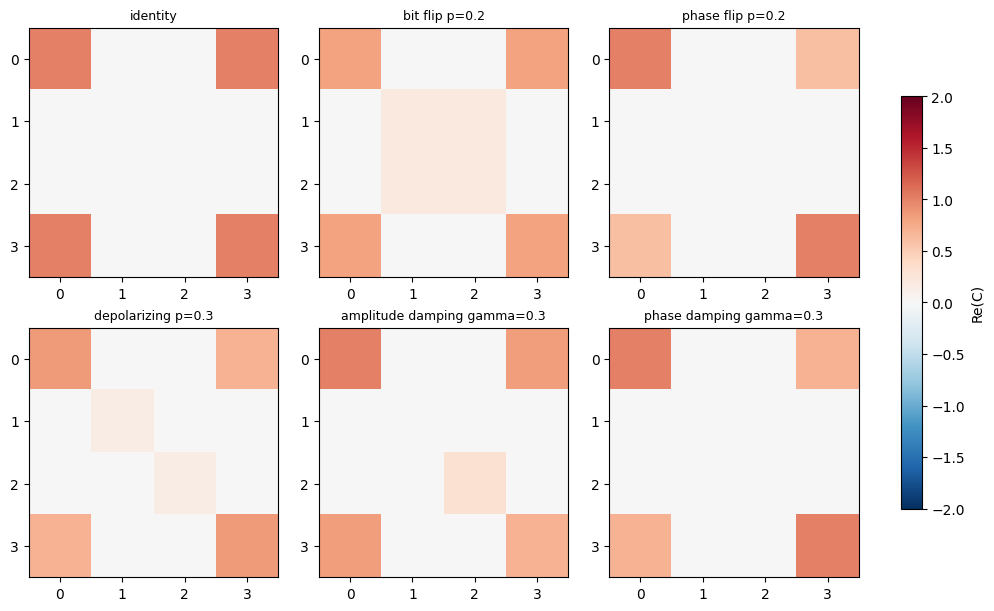
\includegraphics[width=0.94\textwidth]{fig_01_theory_01_cell6.png}
\caption{대표 qubit channel들의 Choi 행렬 실수부. Identity는 rank-1 순수 구조, depolarizing은 대각이 균일해지고, amplitude damping은 비대칭 relaxation 구조. 4.2절의 닫힌 형이 이를 정량적으로 설명한다.}
\label{fig:theory-choi-examples}
\end{figure}

그림 \ref{fig:theory-choi-examples}에서 identity의 Choi는 이상적 최대 얽힘 구조(특정 위치에 큰 결맞음)를, depolarizing은 완전 무질서로 밀리며 구조가 약해짐을 보인다(Bloch의 균일 수축과 동일). amplitude damping은 균일 수축으로 설명되지 않고, 완전 무질서 상태조차 보존하지 않아 TP이지만 비-unital이다.

\begin{property}[TP $\neq$ unital]
$\E$ TP $\iff\Tr_B(C_\E)=I_A$; $\E$ unital $\iff\E(I)=I\iff\Tr_A(C_\E)=I_B$. Bloch에서 ``중심 이동 $\vec t\neq0$''이 곧 비-unital성.
\end{property}

\subsection{수치 검증: ``오차 $10^{-16}$''의 의미}

\begin{mathbox}{기계 정밀도}
배정밀도 단위 반올림 $\varepsilon_{\mathrm{mach}}=2^{-52}\approx2.22\times10^{-16}$. 차이가 $\mathcal O(\varepsilon_{\mathrm{mach}})$이면 ``수치적으로 동일'', $\sim10^{-1}$이면 진짜 차이(예: 5.4절 $-0.27$).
\end{mathbox}

\begin{table}[H]
\centering\small
\begin{tabularx}{\textwidth}{p{0.25\textwidth}p{0.31\textwidth}X}
\toprule
항목 & 관측값 & 해석(근거 식/정리) \\
\midrule
Identity channel & Choi rank $=1$ & $\rank(C_\E)=$ Kraus rank (정리 \ref{thm:cj}); 잡음 없음. \\
Depolarizing $p=0.3$ & min eig $=0.15$, TP=True, unital=True & $\min\mathrm{eig}=p/2=0.15\ge0$(CP); $\vec t=0$(unital). \\
Amplitude damping $\gamma=0.3$ & TP=True, unital=False, rank$=2$ & $\sum K_k^\dagger K_k=I$; $\vec t=(0,0,\gamma)\neq0$. \\
Random round-trip & error $\approx2.56\times10^{-16}$ & Choi$\to$Kraus$\to$작용이 $\mathcal O(\varepsilon_{\mathrm{mach}})$로 일치. \\
Composition check & error $\approx2.48\times10^{-16}$ & $N_{\E_2\circ\E_1}=N_{\E_2}N_{\E_1}$(성질 \ref{prop:compose}). \\
\bottomrule
\end{tabularx}
\caption{이론 파트의 주요 수치 검증 결과}
\label{tab:theory-results}
\end{table}

\begin{remark}
perturbed identity는 에르미트이고 $\Tr_B\approx I$여도 작은 \emph{음의} 고유값 하나로 CP=False가 된다. 정리 \ref{thm:cj}의 $C_\E\succeq0$은 ``거의''를 허용하지 않는다. 이는 5장에서 raw reconstruction을 그대로 믿으면 안 되는 이유다 --- shot noise가 비물리적(음의 고유값) Choi를 만들면 CPTP projection이 필요하다.
\end{remark}

%==================================================================
\section{작업 2 --- Process Tomography와 Choi 재구성}
%==================================================================

\subsection{먼저 알아야 할 것: tomography가 필요한 이유}

이론적 Choi는 코드로 바로 계산되지만, 실제 장치에서 \emph{어떤} 채널이 작용했는지는 알 수 없다. $X$ 게이트를 실행해도 이상적 $X$ 뒤에 amplitude damping·depolarizing·coherent error가 섞일 수 있다.

\begin{conceptbox}{개념: process tomography}
의료 CT처럼 여러 ``각도''의 정보를 합쳐 내부를 복원한다. 알 수 없는 채널에 정보적으로 완전한 입력 $\{\rho_a\}$를 넣고 출력 $\E(\rho_a)$를 측정한 뒤, 선형 관계 $\E(\rho_a)=\Tr_A[(\rho_a^T\otimes I)C_\E]$(정리 \ref{thm:recover})를 $C_\E$에 대해 푼다(\textbf{선형 역산}).
\end{conceptbox}

\begin{definition}[CPTP 사영]
shot noise로 $\widehat C\not\succeq0$일 때 가장 가까운 물리적 채널로 사영:
\[
C^\star=\arg\min_C\onenorm{C-\widehat C}\ \ \text{s.t.}\ \ C\succeq0,\ \Tr_B(C)=I_A,
\]
볼록 최적화(SDP). MLE는 같은 제약 아래 우도 최대화 변형.
\end{definition}

재현성을 위해 실제 하드웨어 대신 \textbf{오프라인 모의 데이터}를 사용했다(파이프라인 검증 목적). 기준 게이트는 그림 \ref{fig:qpt-target-circuits}이며, 잡음은 회로가 아니라 그 뒤의 Choi-레벨 채널로 적용된다.

\begin{conceptbox}{개념: $X$, $H$, CNOT}
\textbf{$X$}: 양자 NOT($|0\rangle\leftrightarrow|1\rangle$). \textbf{$H$}: 균등 중첩을 만드는 아다마르. \textbf{CNOT}: control $q_0$가 $|1\rangle$일 때만 target $q_1$을 뒤집는 \emph{2큐비트} 얽힘 게이트. 앞 둘은 1큐비트, CNOT은 2큐비트라는 점이 뒤 결과 해석의 핵심.
\end{conceptbox}

\begin{figure}[H]
\centering
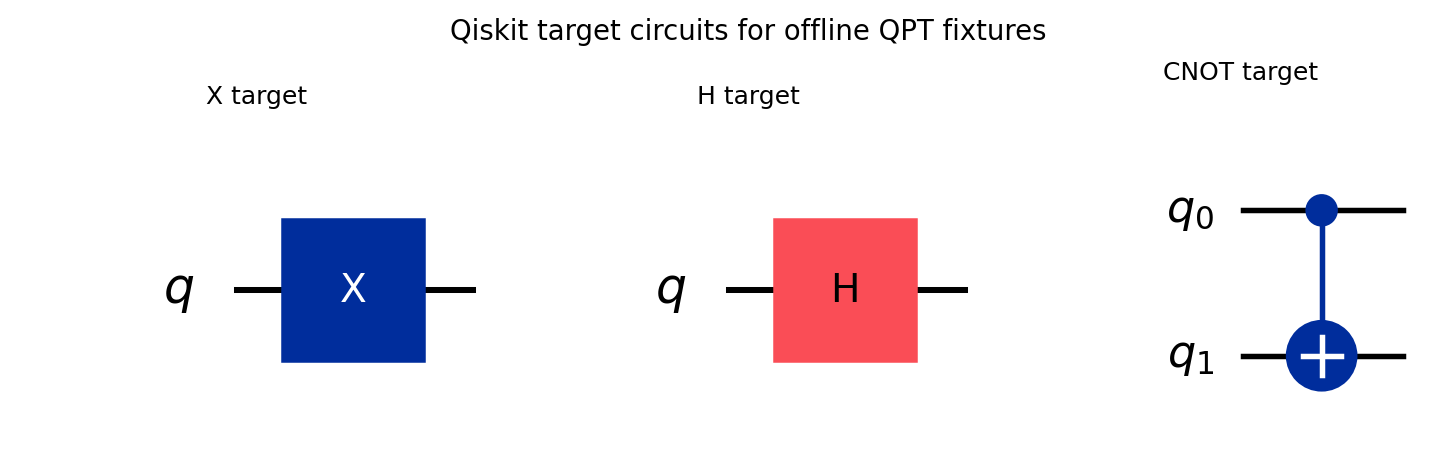
\includegraphics[width=0.92\textwidth]{fig_02_ibm_experiment_00_qiskit_circuits.png}
\caption{Offline QPT fixture의 target circuits. $X,H$는 1큐비트, CNOT은 2큐비트. Noise는 target gate 뒤의 Choi-level channel로 적용.}
\label{fig:qpt-target-circuits}
\end{figure}

\subsection{비교 지표: fidelity와 diamond distance}

\begin{definition}[process fidelity]
$F(\rho,\sigma)=(\Tr\sqrt{\sqrt\rho\sigma\sqrt\rho})^2$. 채널의 process fidelity는 정규화 Choi 상태 $\rho_\E=C_\E/d_A$로 $F_{\mathrm{pro}}(\E,\mathcal F)=F(\rho_\E,\rho_{\mathcal F})$ (entanglement fidelity와 동치).
\end{definition}

\begin{theorem}[average gate fidelity 관계]\label{thm:favg}
$\boxed{F_{\mathrm{avg}}=\dfrac{dF_{\mathrm{pro}}+1}{d+1}}$ (Horodecki--Nielsen).
\end{theorem}

\begin{mathbox}{표 \ref{tab:qpt-results}의 수치 재현}
\begin{align*}
X\,(d{=}2):&\ \tfrac{2(0.959583)+1}{3}=0.973055,\quad
H\,(d{=}2):\ \tfrac{2(0.94)+1}{3}=0.960000,\\
\mathrm{CNOT}\,(d{=}4):&\ \tfrac{4(0.92)+1}{5}=0.936000.
\end{align*}
즉 표의 두 fidelity는 독립 숫자가 아니라 한 공식으로 묶인다.
\end{mathbox}

\begin{definition}[diamond norm]
$\diamondnorm{\Delta}=\max_{\rho\in\Dens(\Hcal_A\otimes\Hcal_R)}\onenorm{(\Delta\otimes\id_R)(\rho)}$, $\dim\Hcal_R=\dim\Hcal_A$ (최댓값은 순수 상태에서). half-diamond distance $=\tfrac12\diamondnorm{\E_0-\E_1}$.
\end{definition}

\begin{intuitionbox}
\textbf{fidelity 대 diamond:} fidelity는 Choi \emph{상태}의 평균적 겹침, diamond는 \emph{최악의 입력}(얽힘 허용)에서의 차이. $X$가 $F_{\mathrm{pro}}=0.96$로 평균적으로 비슷해도 half-diamond $=0.08\neq0$로 ``최악에서는 구별됨''.
\end{intuitionbox}

\subsection{이상적 Choi 대 재구성된 Choi}

\begin{figure}[H]
\centering
\begin{subfigure}{0.48\textwidth}\centering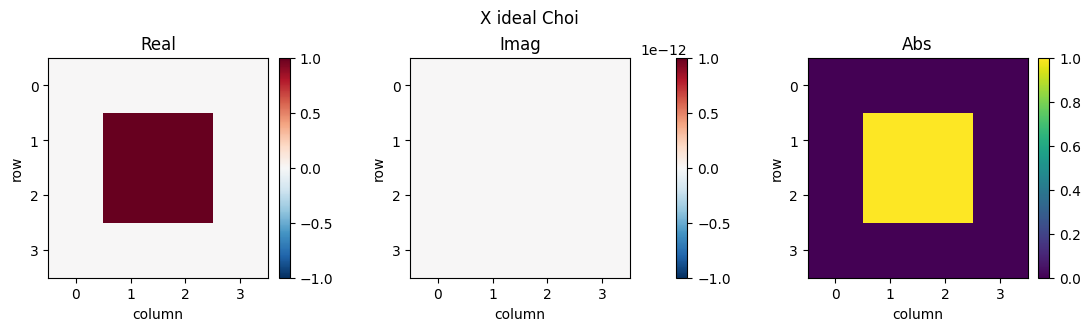
\includegraphics[width=\textwidth]{fig_02_ibm_experiment_01_cell20.png}\caption{$X$ ideal Choi}\end{subfigure}\hfill
\begin{subfigure}{0.48\textwidth}\centering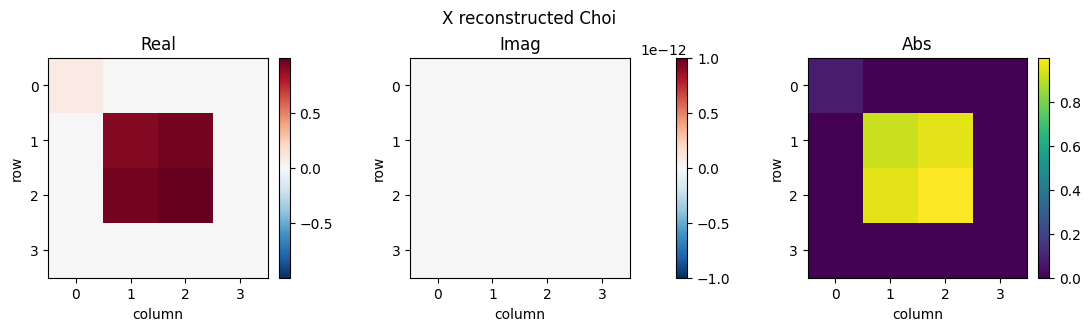
\includegraphics[width=\textwidth]{fig_02_ibm_experiment_02_cell20.png}\caption{$X$ reconstructed Choi}\end{subfigure}
\caption{$X$의 ideal/reconstructed Choi. 큰 구조는 유지되되 ideal pattern을 벗어난 작은 성분 출현 --- 이상적 unitary에 잡음이 더해진 형태.}
\label{fig:qpt-x-choi}
\end{figure}

두 행렬이 완전히 같다면 $F_{\mathrm{pro}}=1$, half-diamond $=0$이어야 한다. 실측은 $F_{\mathrm{pro}}=0.959583$, half-diamond $=0.080000$으로, ``평균적 유사 / 최악의 차이'' 구도를 보여준다.

\begin{figure}[H]
\centering
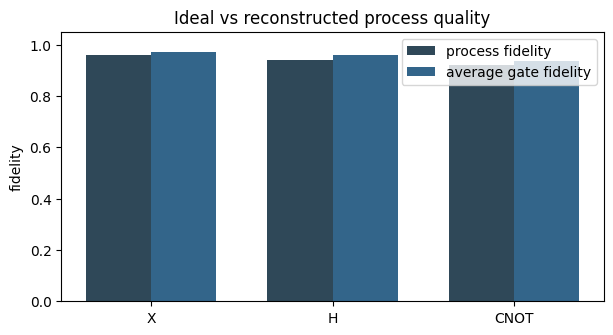
\includegraphics[width=0.74\textwidth]{fig_02_ibm_experiment_10_cell24.png}
\caption{$X,H,$CNOT의 process/average gate fidelity. 모두 $<1$(잡음 존재), CNOT 최저.}
\label{fig:qpt-fidelity-bars}
\end{figure}

\begin{remark}[차원이 커지면 왜 나빠지나]
CNOT은 2큐비트라 $C_\E\in\Lin(\mathbb C^{16})$, 전역 depolarizing의 Pauli error 갈래 수 $d^2-1=15$(1큐비트의 $3$보다 많음). 같은 세기라도 오차가 더 많은 방향으로 분산되어 $F_{\mathrm{pro}}$가 낮아진다.
\end{remark}

\subsection{잡음의 방향성: Bloch 아핀 진단}

\begin{definition}[잔차 채널의 아핀 진단]
잔차를 $\vec r\mapsto M\vec r+\vec t$로 보고 $M=U\Sigma V^\dagger$, $\Sigma=\mathrm{diag}(s_1,s_2,s_3)$. 분류:
\[
\|\vec t\|_2>\tau\Rightarrow\text{relaxation-like},\quad
\|\vec t\|_2\approx0\ \&\ \mathrm{spread}(s_i)\approx0\Rightarrow\text{depolarizing-like},
\]
$\mathrm{spread}=\max_i s_i-\min_i s_i$, $\tau=0.05$.
\end{definition}

\begin{figure}[H]
\centering
\begin{subfigure}{0.47\textwidth}\centering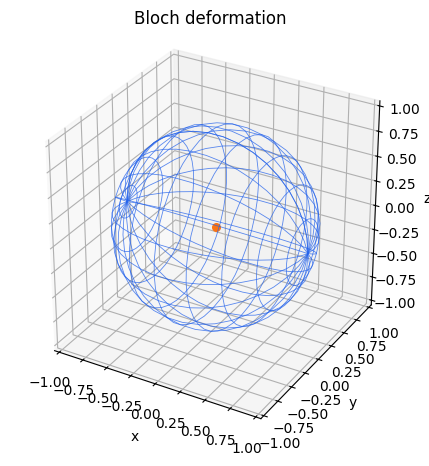
\includegraphics[width=0.82\textwidth]{fig_02_ibm_experiment_07_cell22.png}\caption{$X$ reconstructed}\end{subfigure}\hfill
\begin{subfigure}{0.47\textwidth}\centering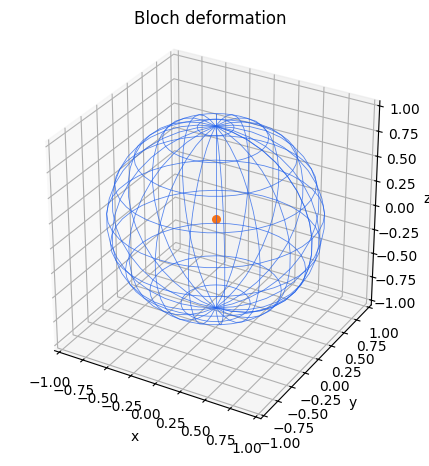
\includegraphics[width=0.82\textwidth]{fig_02_ibm_experiment_08_cell22.png}\caption{$H$ reconstructed}\end{subfigure}
\caption{재구성된 1큐비트 채널의 Bloch 변형. depolarizing-like는 균일 수축($\vec t\approx0$), amplitude-damping-like는 중심 이동($\vec t\neq0$). fidelity 숫자만으로 안 보이는 방향성을 드러낸다.}
\label{fig:qpt-bloch}
\end{figure}

\begin{table}[H]
\centering\small
\begin{tabularx}{\textwidth}{lcccX}
\toprule
Gate & $\|\vec t\|_2$ & SV spread & Mean shrinkage & 진단 근거 \\
\midrule
$X$ & 0.07999965 & 0.03916625 & 0.94611071 & $\|\vec t\|_2>0.05\Rightarrow$ relaxation-like. \\
$H$ & $1.999\times10^{-15}$ & $1.999\times10^{-12}$ & 0.92000000 & $\|\vec t\|_2,\mathrm{spread}\approx\mathcal O(\varepsilon)\Rightarrow$ isotropic depolarizing-like. \\
\bottomrule
\end{tabularx}
\caption{1큐비트 재구성 채널의 Bloch affine 진단. $H$의 $10^{-15},10^{-12}$는 ``$0$''(4.3절).}
\label{tab:qpt-bloch-diagnostics}
\end{table}

따라서 tomography는 세 가지를 함께 보아야 한다: heatmap(구조적 차이), fidelity(한 숫자 요약), Bloch(물리적 잡음 모양). 종합이 표 \ref{tab:qpt-results}이다.

\begin{table}[H]
\centering\small
\begin{tabularx}{\textwidth}{lcccX}
\toprule
Gate & $F_{\mathrm{pro}}$ & $F_{\mathrm{avg}}$ & Half-diamond & 진단 \\
\midrule
$X$ & 0.959583 & 0.973055 & 0.080000 & amplitude-damping-like relaxation \\
$H$ & 0.940000 & 0.960000 & 0.060000 & depolarizing-like isotropic shrinkage \\
CNOT & 0.920000 & 0.936000 & 0.080000 & stochastic global depolarizing-like noise \\
\bottomrule
\end{tabularx}
\caption{Offline simulated QPT 결과 ($F_{\mathrm{avg}}$는 정리 \ref{thm:favg}로 유도).}
\label{tab:qpt-results}
\end{table}

\begin{remark}[비물리적 재구성]
선형 역산 perturbation의 최소 고유값 $-0.270000$은 $\mathcal O(\varepsilon_{\mathrm{mach}})$가 아닌 진짜 음수(정리 \ref{thm:cj} 위반). CPTP 사영(5.1절)으로 $C^\star\succeq0$을 회복해야 한다 --- 결과를 예쁘게 만드는 후처리가 아니라 물리 법칙(고유값 $\ge0$)의 회복.
\end{remark}

%==================================================================
\section{작업 3 --- Channel Discrimination, diamond norm, SDP}
%==================================================================

\subsection{먼저 알아야 할 것: ``구별''은 ``비슷함''과 다른 문제}

fidelity는 ``평균적 유사도''다. 그러나 ``두 채널을 실제로 얼마나 잘 \emph{구별}하는가''는 별개다. 동전을 던져 $\E_0,\E_1$ 중 하나를 주면, 원하는 입력으로 측정해 어느 쪽인지 맞히는 게임을 생각하자.

\begin{theorem}[Holevo--Helstrom]\label{thm:helstrom}
사전확률 $\tfrac12$씩으로 두 상태 $\rho_0,\rho_1$ 구별의 최적 성공확률은
\[
p_{\mathrm{succ}}^{\max}=\tfrac12+\tfrac14\onenorm{\rho_0-\rho_1}=\tfrac12+\tfrac12T(\rho_0,\rho_1),
\]
최적 측정은 $\rho_0-\rho_1$의 양/음 고유공간 사영. $T(\rho_0,\rho_1)=\tfrac12\onenorm{\rho_0-\rho_1}$.
\end{theorem}
\begin{proof}[증명 개요]
POVM $\{M,I-M\}$의 성공확률 $\tfrac12+\tfrac12\Tr[M\Delta]$, $\Delta=\Delta_+-\Delta_-$. $\Tr[M\Delta]\le\Tr\Delta_+=\tfrac12\onenorm\Delta$, $M=\Delta_+$ 사영에서 등호.
\end{proof}

\begin{theorem}[채널 구별과 diamond norm]\label{thm:chandisc}
$\E_0,\E_1$을 한 번 사용해 구별하는 최적 성공확률(참조계 허용)은
\[
\boxed{p_{\mathrm{succ}}^{\max}=\tfrac12+\tfrac14\diamondnorm{\E_0-\E_1}.}
\]
\end{theorem}
\begin{proof}[증명 개요]
입력 $|\psi\rangle\in\Hcal_A\otimes\Hcal_R$에 정리 \ref{thm:helstrom}을 적용하면 성공확률 $\tfrac12+\tfrac14\onenorm{(\Delta\otimes\id_R)(|\psi\rangle\langle\psi|)}$, $|\psi\rangle$로 최대화 $=\diamondnorm\Delta$.
\end{proof}

\begin{mathbox}{왜 참조계(ancilla)가 도움이 되는가}
$\diamondnorm{}$의 최댓값이 \emph{얽힌} $|\psi\rangle$에서 달성될 수 있기 때문이다. 단독 입력만 쓰면 더 작은 값만 얻는다:
\[
\max_{\rho\in\Dens(\Hcal_A)}\onenorm{\Delta(\rho)}\ \le\ \diamondnorm{\Delta},
\]
부등호가 엄격할 수 있다 --- 표 \ref{tab:sdp-results}의 $0.750\to0.875$ 향상의 근원.
\end{mathbox}

\begin{theorem}[Watrous SDP]\label{thm:sdp}
$\Delta$의 Choi $J=C_\Delta$($A$ 입력)에 대해
\[
\diamondnorm{\Delta}=\max_{W,\rho}\langle J,W\rangle\quad\text{s.t.}\quad0\preceq W\preceq\rho\otimes I_B,\ \rho\in\Dens(\Hcal_A),
\]
변수 $W\succeq0,\rho\succeq0$의 볼록 문제로 효율적으로 풀린다 (Watrous 2009/2012).
\end{theorem}

\begin{conceptbox}{개념: SDP가 자연스러운 이유}
``물리적으로 가능한'' 대상은 모두 $\succeq0$ 제약으로 표현되므로, ``최적 전략'' 찾기가 $\succeq0$ 아래 선형 목적 최적화(SDP)가 된다. \textbf{Choi 행렬 $J$가 SDP의 입력 데이터}라는 점이 핵심 --- Choi가 operational 양과 직결되는 통로.
\end{conceptbox}

\subsection{수치 결과}

\begin{figure}[H]
\centering
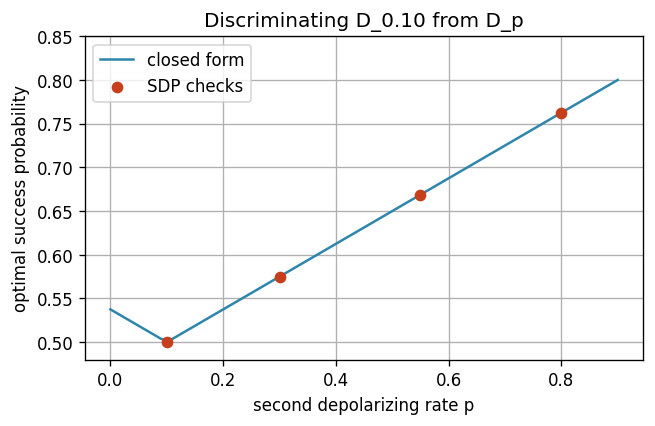
\includegraphics[width=0.72\textwidth]{fig_03_sdp_discrimination_01_cell9.png}
\caption{Depolarizing 매개변수 차이에 따른 구별 성공확률. 차이$\to0$이면 $p\to\tfrac12$(찍기), 커지면 정리 \ref{thm:chandisc}로 $p$ 증가.}
\label{fig:sdp-depolarizing}
\end{figure}

\begin{figure}[H]
\centering
\begin{subfigure}{0.48\textwidth}\centering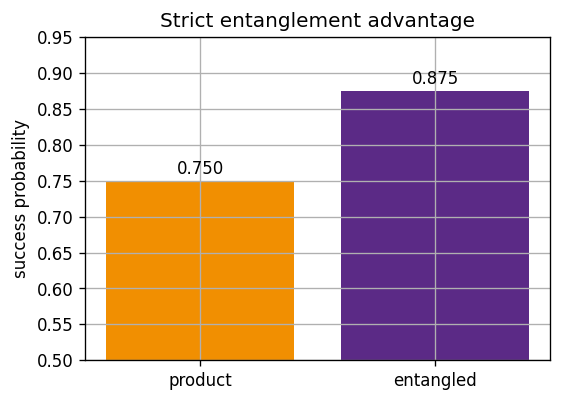
\includegraphics[width=\textwidth]{fig_03_sdp_discrimination_04_cell18.png}\caption{Product vs entangled}\end{subfigure}\hfill
\begin{subfigure}{0.48\textwidth}\centering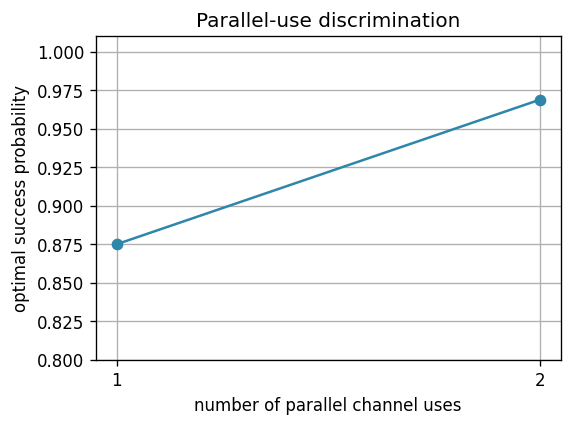
\includegraphics[width=\textwidth]{fig_03_sdp_discrimination_05_cell21.png}\caption{Parallel use}\end{subfigure}
\caption{얽힘과 반복 사용의 이점. product $0.750000$, ancilla-assisted $0.875000$, 2-shot parallel $0.968750$.}
\label{fig:sdp-advantage}
\end{figure}

단독과 얽힌 입력의 차이는 단순 계산상 차이가 아니라 \textbf{operational advantage}다. 참조계와 얽힘을 만들면 채널 작용이 합동 상태의 상관에도 흔적을 남겨, 그 추가 정보로 성공확률이 오른다($0.75\to0.875$).

\begin{property}[병렬 사용은 곱 채널의 diamond norm]
$n$번 병렬 사용 전략의 성공확률은 $\tfrac12+\tfrac14\diamondnorm{\E_0^{\otimes n}-\E_1^{\otimes n}}$로 차이가 누적. 다만 차원이 $d_A^n$으로 지수 증가하여 SDP 비용 급증.
\end{property}

\begin{table}[H]
\centering
\begin{tabular}{lcc}
\toprule
전략 & 성공확률 & 근거 \\
\midrule
Bit-flip closed-form 검증 & 0.625000 & 해석적 $\diamondnorm{}$와 SDP(정리 \ref{thm:sdp}) 일치 → 구현 신뢰성. \\
Product input & 0.750000 & $\max_\rho\onenorm{\Delta(\rho)}$ (참조계 없음). \\
Ancilla-assisted input & 0.875000 & 전체 $\diamondnorm{\Delta}$ (정리 \ref{thm:chandisc}). \\
2-shot parallel & 0.968750 & 차이 누적. \\
\bottomrule
\end{tabular}
\caption{SDP 기반 channel discrimination 결과}
\label{tab:sdp-results}
\end{table}

첫 줄($0.625$)은 손으로 풀리는 bit-flip(예제 \ref{ex:bitflip}의 채널)의 해석적 diamond norm과 SDP 수치 일치로 구현을 검증한다. $0.750\to0.875\to0.969$의 단조 증가는 ``참조계 없음 $\to$ 얽힘 $\to$ 반복''에 대응한다.

%==================================================================
\section{작업 4 --- Non-Markovian Dynamics와 Quantum Combs}
%==================================================================

\subsection{먼저 알아야 할 것: 단일 시점 채널의 한계}

지금까지의 Choi는 \emph{하나의} 입력-출력 관계다. 그러나 시간 과정에서 계가 환경과 여러 번 상호작용하고 그 환경이 다음 시점에도 \emph{기억}을 남기면 단일 채널로 설명되지 않는다.

\begin{conceptbox}{개념: Markovian 대 non-Markovian}
\textbf{Markovian}은 기억 없는 과정 --- 환경으로 새어 나간 정보가 돌아오지 않는다. \textbf{non-Markovian}은 환경에 저장된 정보가 계로 \emph{되돌아올} 수 있다. 각 시점 marginal이 멀쩡한 CPTP라도 시점 간 상관이 남으면 전체는 ``기억 없는 곱''으로 분해되지 않는다.
\end{conceptbox}

\begin{definition}[동역학 사상과 CP-divisibility]
시간 채널 족 $\{\Lambda(t)\}$($\Lambda(0)=\id$)에서 중간 전파자 $V(t,s)$를 $\Lambda(t)=V(t,s)\Lambda(s)$로 정의. 모든 $t\ge s$에서 $V(t,s)$가 CP이면 \textbf{CP-divisible}(Markovian).
\end{definition}

\begin{property}[CPTP의 trace-distance 수축성]\label{prop:contract}
CPTP $\Lambda$와 두 상태에 대해 $T(\Lambda\rho,\Lambda\sigma)\le T(\rho,\sigma)$. 즉 물리적(CP) 진화는 구별 가능성을 증가시키지 못한다.
\end{property}

\begin{intuitionbox}
\textbf{직관(성질 \ref{prop:contract}의 위력):} trace distance가 \emph{다시 증가}하면, 그 구간의 중간 전파자는 CP일 수 없다 --- 정보가 환경에서 계로 되돌아온 것. 이것이 기억 효과의 신호다.
\end{intuitionbox}

\begin{conceptbox}{개념: trace distance와 BLP measure}
\textbf{trace distance} $T=\tfrac12\onenorm{\rho-\sigma}$는 두 상태 구별 가능성(0=구별 불가). 잡음은 보통 $T$를 단조 감소시키지만, 재증가하면 기억 효과의 증거다.
\end{conceptbox}

\begin{definition}[BLP measure]
$\sigma(t)=\frac{d}{dt}T(\Lambda(t)\rho_1,\Lambda(t)\rho_2)$일 때 $\mathcal N_{\mathrm{BLP}}=\max_{\rho_1,\rho_2}\int_{\sigma(t)>0}\sigma(t)\,dt$. $>0$이면 non-Markovian.
\end{definition}

\begin{conceptbox}{개념: RHP-style witness}
RHP는 중간 전파자 $V(t+\epsilon,t)$의 CP성을 직접 본다. $g(t)=\lim_{\epsilon\to0^+}\frac1\epsilon(\onenorm{(\id\otimes V(t+\epsilon,t))|\Omega\rangle\langle\Omega|}-1)$이 $V$가 CP인 동안 $0$, 깨지면 $>0$. 적분이 RHP-style witness. BLP가 ``정보 역류''를, RHP가 ``중간 단계 비-CP''를 본다.
\end{conceptbox}

\begin{figure}[H]
\centering
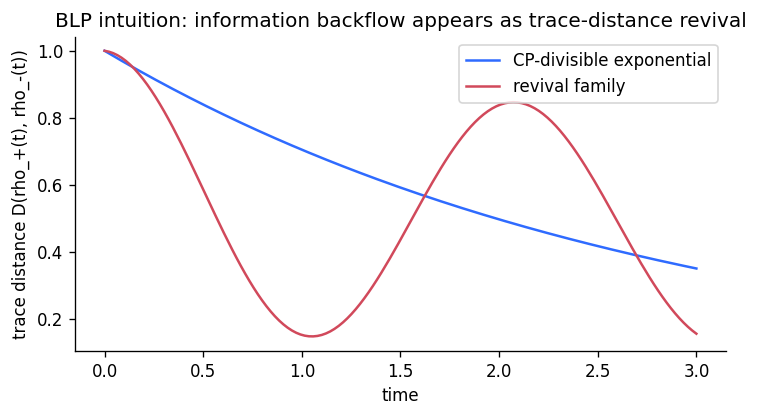
\includegraphics[width=0.76\textwidth]{fig_04_quantum_combs_01_cell7.png}
\caption{trace distance의 시간 변화. Markovian dephasing은 단조 감소($\sigma\le0$, 성질 \ref{prop:contract}와 부합), revival dephasing은 재증가($\sigma>0$) → $\mathcal N_{\mathrm{BLP}}>0$. 정보가 environment에서 system으로 되돌아옴.}
\label{fig:comb-trace-distance}
\end{figure}

\subsection{구조적 증거: comb와 memoryless product}

trace distance 곡선만으로는 다중 시점 과정 \emph{전체}의 구조를 못 본다. 전체 two-use 과정을 하나의 comb로 놓고 기억 없는 곱과 비교한다.

\begin{conceptbox}{개념: quantum comb}
여러 time slot의 입력-출력을 하나의 큰 ``Choi 같은'' 연산자로 묶은 것. 이름이 ``빗''인 것은 시간 축을 따라 단자(이빨)가 늘어선 모양 때문. 단일 채널에선 안 보이는 시간 상관·기억 잔여물을 드러낸다.
\end{conceptbox}

\begin{definition}[quantum comb의 인과 위계]
$N$-comb은 $\bigotimes_k\Hcal_k$(번갈아 in/out) 위 $C\succeq0$. 2-comb은
\[
\Tr_3 C=I_2\otimes C^{(1)},\qquad \Tr_1 C^{(1)}=I_0
\]
를 만족(Chiribella--D'Ariano--Perinotti). 정리 \ref{thm:cj}의 TP($\Tr_B C_\E=I_A$)를 여러 시점으로 확장한 것.
\end{definition}

\begin{definition}[link product과 상관 노름]
comb 합성은 공유 계의 부분 대각합·전치를 결합한 \textbf{link product} $\star$. 기억 없는 과정은 $C_{\mathrm{prod}}=\bigotimes_k C^{(k)}$로 분해되고, 상대 상관 노름
\[
\eta=\frac{\onenorm{C-C_{\mathrm{prod}}}}{\onenorm{C}}
\]
이 $\neq0$이면 시점 간 상관(기억) 존재.
\end{definition}

\begin{conceptbox}{개념: collision model}
계가 환경 입자들과 차례로 ``충돌''하는데, \emph{같은 환경을 재사용}하면 첫 충돌의 흔적이 다음 충돌에 영향을 준다 --- ``환경 재사용''이 기억의 원천.
\end{conceptbox}

\begin{figure}[H]
\centering
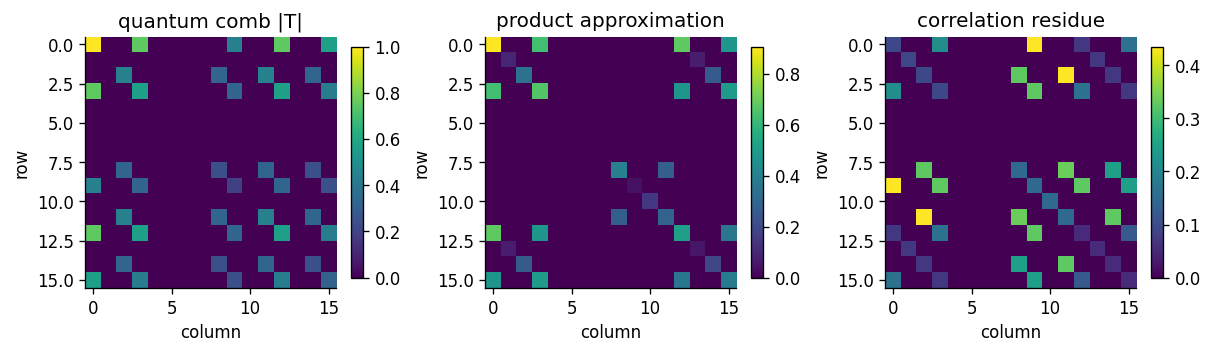
\includegraphics[width=0.92\textwidth]{fig_04_quantum_combs_02_cell10.png}
\caption{Two-use collision model의 comb(좌), memoryless product(중), 차이(우). 차이$\neq0\Rightarrow$ 시점 간 상관 존재 --- 독립적 두 채널의 연속으로 설명 안 됨.}
\label{fig:comb-correlation}
\end{figure}

\begin{mathbox}{collision model의 수치 검증}
$C\in\Lin(\mathbb C^{16})$, 최소 고유값 $-1.774\times10^{-16}=\mathcal O(\varepsilon_{\mathrm{mach}})\Rightarrow C\succeq0$(물리적). 인과 위계=True. 그러나 곱 분해 가능성=False, $\eta=\onenorm{C-C_{\mathrm{prod}}}/\onenorm{C}\approx0.5307\neq0$. \textbf{이 $\eta\neq0$이 기억 효과의 정량적 핵심 증거.}
\end{mathbox}

기억은 각 시점 marginal이 \emph{이상해서}가 아니라 \emph{시점 간 상관}에서 나온다. 다음 그림이 이를 보인다.

\begin{figure}[H]
\centering
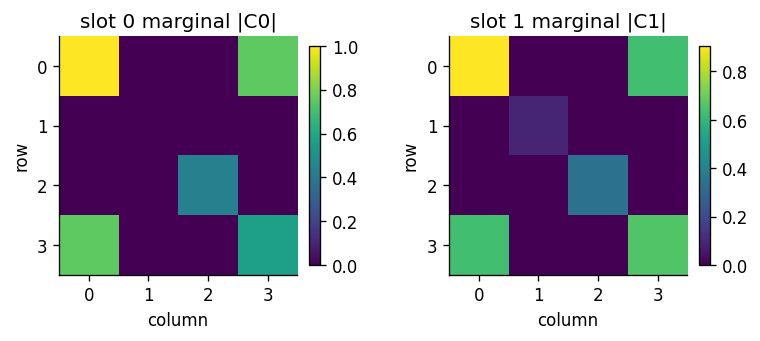
\includegraphics[width=0.72\textwidth]{fig_04_quantum_combs_03_cell13.png}
\caption{각 slot의 marginal Choi. 개별로는 정상적 1단계 채널이나 곱만으로 전체 comb 복원 불가($\eta\neq0$). 매 시점 멀쩡한 채널을 얻어도 전체가 Markovian이라 결론낼 수 없다.}
\label{fig:comb-marginals}
\end{figure}

\begin{table}[H]
\centering
\begin{tabular}{lcc}
\toprule
Channel family & BLP grid estimate & RHP-style grid witness \\
\midrule
Exponential dephasing & 0.000000 & 0.000000 \\
Revival dephasing & 0.699240 & 0.896321 \\
\bottomrule
\end{tabular}
\caption{비마르코프성 witness 결과. 정의가 다른 두 진단이 같은 결론.}
\label{tab:nonmarkov-results}
\end{table}

exponential dephasing은 $\mathcal N_{\mathrm{BLP}}=0$, RHP$=0$(CP-divisible). revival dephasing은 둘 다 양수로, \emph{서로 독립적인 두 measure}가 동일하게 non-Markovian을 가리킨다 --- 결과의 robust함.

%==================================================================
\section{작업 5 --- Interactive Widget과 조건의 시각적 동치}
%==================================================================

Widget은 정리 \ref{thm:cj}의 두 조건을 \emph{실시간으로} 보여준다. 수식으로 $C_\E\succeq0$, $\Tr_B(C_\E)=I_A$는 간단해 보이지만, 채널 작용에서 어떤 모양인지 떠올리기는 어렵다. 매개변수를 움직이면 다음이 동시에 갱신된다.
\[
\underbrace{\text{Choi eigenspectrum}}_{C_\E\succeq0?\ (\text{CP})},\quad
\underbrace{\Tr_B(C_\E)}_{=I_A?\ (\text{TP})},\quad
\underbrace{\text{Kraus }\{K_k\}}_{\text{정리 \ref{thm:cj}}},\quad
\underbrace{\vec r\mapsto M\vec r+\vec t}_{\text{Bloch}}.
\]

앞 네 작업은 Choi를 따로 사용했지만, widget은 이들을 \emph{한 화면에서 연결}한다. amplitude damping을 고르면 Choi 패턴·고유값뿐 아니라 Bloch가 어느 방향으로 변형되는지도 동시에 보인다.

\begin{figure}[H]
\centering
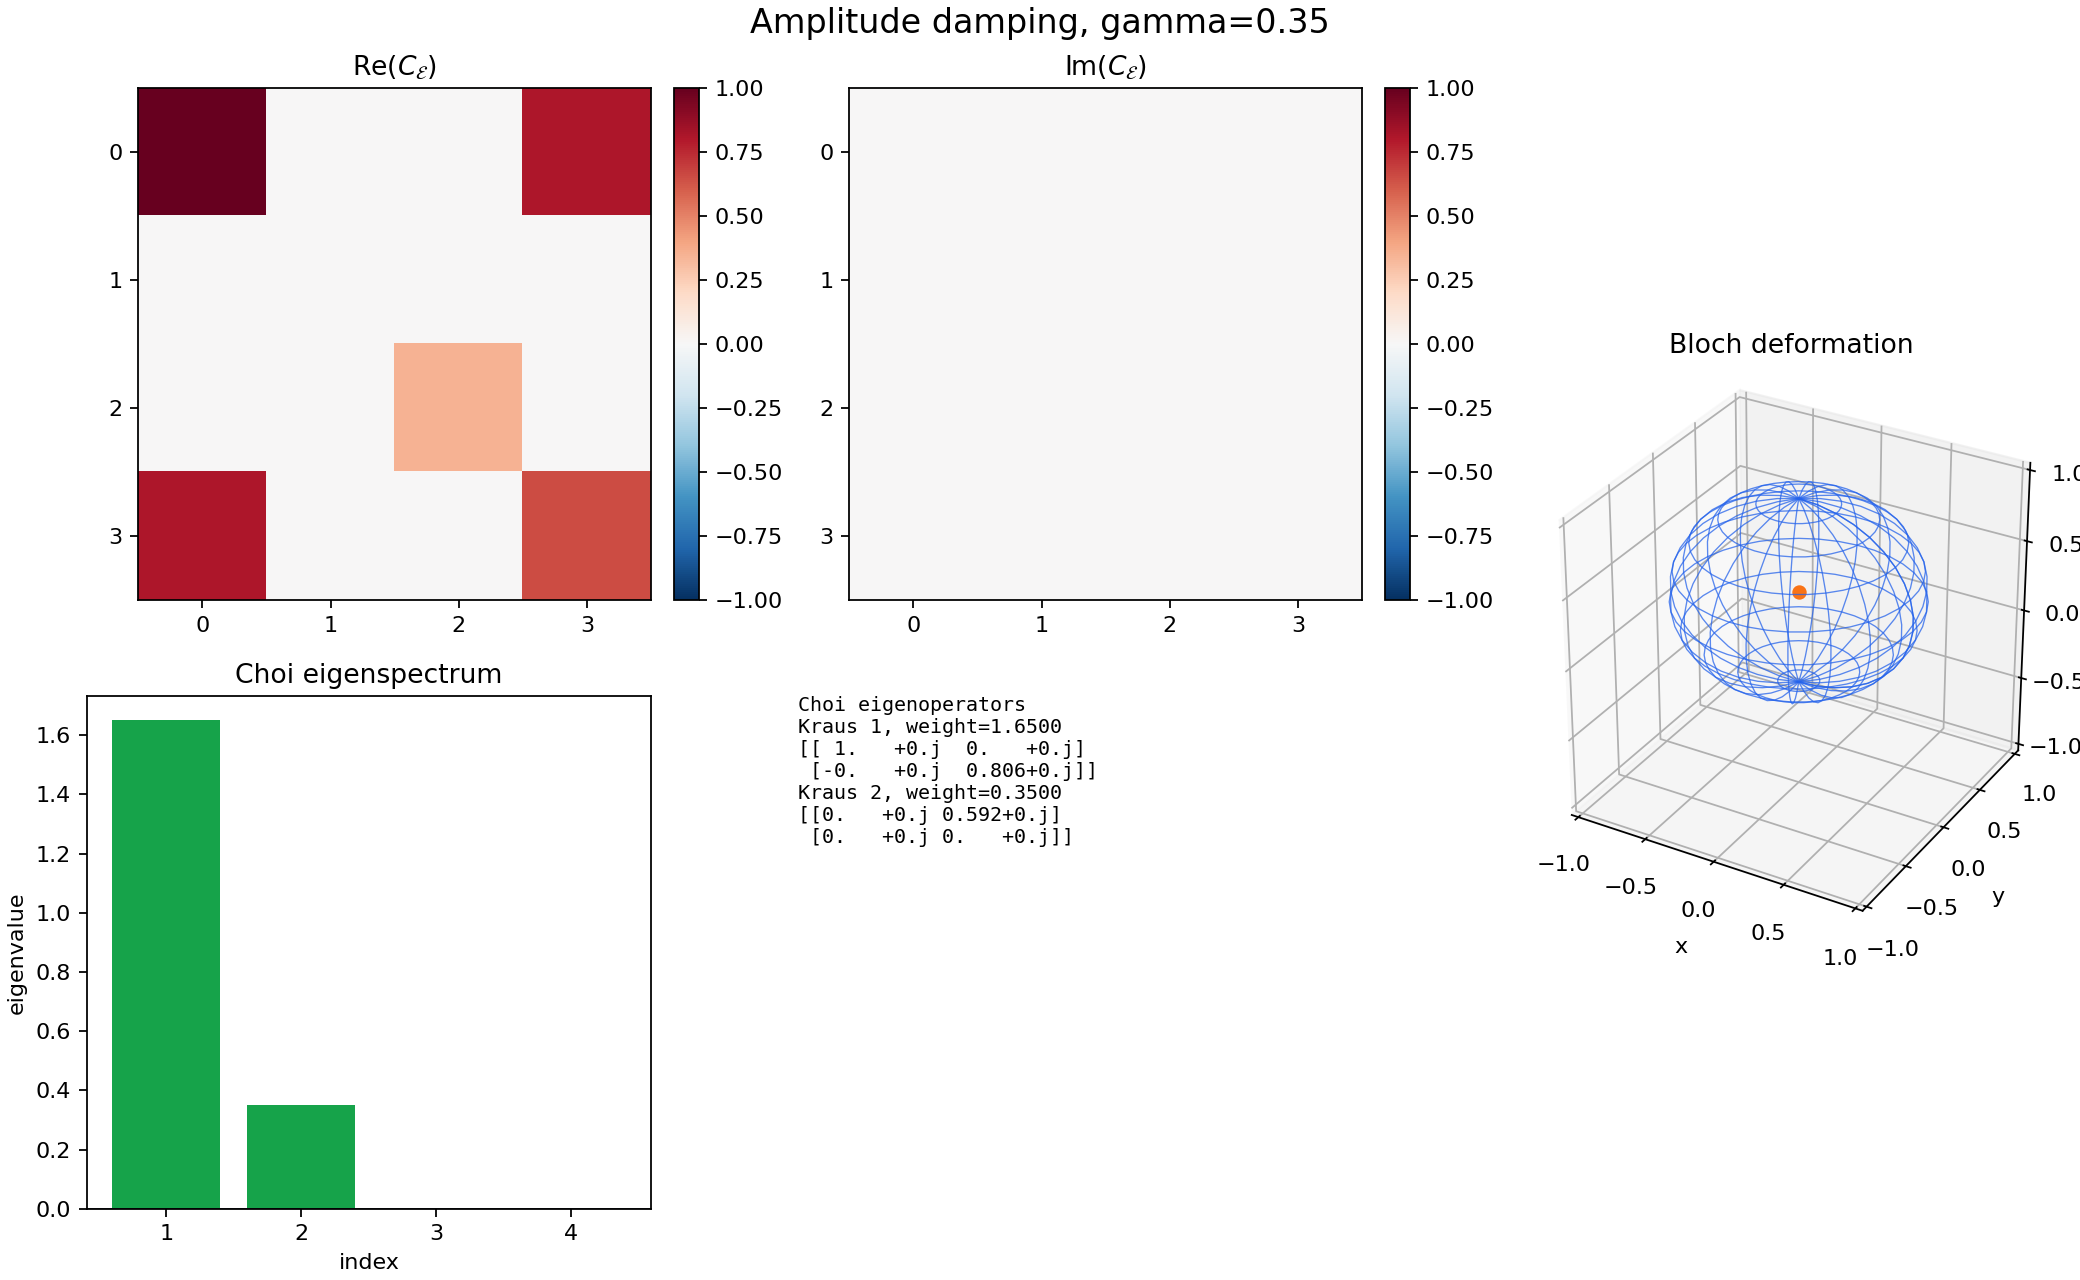
\includegraphics[width=0.94\textwidth]{fig_widget_dashboard.png}
\caption{amplitude damping 예시. Choi 실수부/허수부/절댓값(좌), Choi 고유값과 Bloch 변형(우). $\vec t=(0,0,\gamma)\neq0$이라 중심이 이동 --- 비-unital성의 시각적 표현(4.2절 상자).}
\label{fig:widget-dashboard}
\end{figure}

\begin{property}[CP 경계의 시각적 신호]
매개변수를 CP 영역 밖으로 옮기면 $C_\E$에 음의 고유값이 나타난다(정리 \ref{thm:cj} 위반). 성분 변화는 작아 보여도 $\min\mathrm{eig}(C_\E)<0$이 되는 순간 비물리적 --- 4.3절 perturbed identity, 5.4절 비물리적 재구성과 같은 현상의 대화형 버전.
\end{property}

따라서 widget은 단순 시각화가 아니라 작업 1의 CP/TP 판정, 작업 2의 잡음 진단($M,\vec t$), 작업 3의 채널 차이를 한 화면에서 잇는 마지막 연결 고리다.

%==================================================================
\section{통합 해석과 한계}
%==================================================================

\subsection{Choi 행렬은 어떻게 다섯 작업을 하나로 묶었나}

가장 중요한 통합점은 Choi 행렬이 \emph{공통 인터페이스}로 작동했다는 것이다. 작업 1에서 표현 변환·CP/TP 판정의 기준, 작업 2에서 재구성 대상이자 fidelity·잡음 진단의 출발점, 작업 3에서 두 Choi의 차이가 SDP 입력, 작업 4에서 다중 시점 comb로 확장, 작업 5에서 시각적 대시보드.

\begin{longtable}{p{0.15\textwidth}p{0.40\textwidth}p{0.33\textwidth}}
\toprule
파트 & Choi 행렬의 역할 & 핵심 식 \\
\midrule
이론 & 표현 변환·물리성 판정 & $C_\E\succeq0$(CP), $\Tr_B C_\E=I_A$(TP) \\
Tomography & 재구성 대상 & $\E(\rho)=\Tr_A[(\rho^T\otimes I)C_\E]$, $F_{\mathrm{avg}}=\frac{dF_{\mathrm{pro}}+1}{d+1}$ \\
SDP & 최적화 입력 데이터 & $p=\tfrac12+\tfrac14\diamondnorm{\E_0-\E_1}$ \\
Combs & 다중 시점 확장 & $\Tr_3 C=I_2\otimes C^{(1)}$, $\eta=\onenorm{C-C_{\mathrm{prod}}}/\onenorm{C}$ \\
Widget & 조건의 동치 표현 & $\min\mathrm{eig}(C_\E)\gtrless0$ \\
\bottomrule
\caption{Choi 표현의 통합적 역할}
\label{tab:integration}
\end{longtable}

종합하면 Choi 행렬은 단일 선형 대상 $C_\E\in\Lin(\Hcal_A\otimes\Hcal_B)$ 위에서 물리성을 \emph{판정}하고($\succeq0$, $\Tr_B=I$), 재구성의 \emph{대상}이 되며, 두 행렬 차이가 최적화의 \emph{입력}($\diamondnorm{}$)이 되고, 다중 시점으로 \emph{확장}된다(comb). 같은 표현을 끝까지 유지한 덕에 다섯 작업이 하나의 식 체계로 연결되었다.

\subsection{무엇을 조심해야 하는가}

\begin{remark}[규모의 한계]
$C_\E$의 크기는 $d_Ad_B$, SDP 변수는 $\mathcal O((d_Ad_B)^2)$. $N$-comb은 $\prod_k d_k$로 \emph{지수} 증가($\eta$ 계산 비용 포함). 대규모로 가려면 대칭성, tensor network, randomized benchmarking 같은 압축이 필요하다.
\end{remark}

\begin{remark}[하드웨어 주장 금지]
tomography 수치는 offline simulated fixture 기반이다. 표의 $F_{\mathrm{pro}}$/diamond 값을 실제 IBM 하드웨어 성능으로 해석하면 안 된다. 하드웨어 주장에는 backend 이름, 보정 시각, shot 수, job ID, raw count, 불확실성 추정이 필요하다. 본 결과는 분석 파이프라인·해석 방식의 검증으로 보아야 한다.
\end{remark}

%==================================================================
\section{결론}
%==================================================================

본 프로젝트는 Choi 표현이 왜 강력한 도구인지를 직관과 수식으로 확인했다. 핵심은 \textbf{Choi--Jamio{\l}kowski 동형사상}(정리 \ref{thm:cj})으로,
\[
\E\text{ CP}\iff C_\E\succeq0,\qquad \E\text{ TP}\iff\Tr_B(C_\E)=I_A
\]
이 모든 작업의 토대가 되었다.

\begin{itemize}
  \item \textbf{이론(작업 1):} Kraus/Choi/Stinespring/natural이 $\mathcal O(\varepsilon_{\mathrm{mach}})$로 일관 변환됨을 확인.
  \item \textbf{Tomography(작업 2):} 재구성 Choi가 fidelity($F_{\mathrm{avg}}=\frac{dF_{\mathrm{pro}}+1}{d+1}$), diamond distance, Bloch 변형으로 잡음의 \emph{크기와 방향}을 드러냄.
  \item \textbf{SDP(작업 3):} $p=\tfrac12+\tfrac14\diamondnorm{\cdot}$로 diamond norm이 구별 성공확률과 직결되고, 얽힘·반복이 성능을 높임($0.75\to0.875\to0.969$).
  \item \textbf{Quantum comb(작업 4):} marginal이 멀쩡해도 $\eta\neq0$이면 전체에 기억 상관이 남음을 BLP/RHP로 확인.
  \item \textbf{Widget(작업 5):} 조건들을 한 화면에서 보여 수식과 직관의 간격을 줄임.
\end{itemize}

특히 CP 조건이 ``고유값 $\ge0$''으로, TP 조건이 ``부분 대각합 $=I$''로 바뀐다는 점이 계산·해석 모두에서 큰 장점이다. 다만 계가 커질수록 $C_\E$와 SDP의 크기가 급증하므로, 향후 더 효율적인 표현과 근사가 필요하다.

\appendix
%==================================================================
\section{부록 A --- 한눈에 보는 요약 치트시트}
%==================================================================

\begin{longtable}{p{0.20\textwidth}p{0.36\textwidth}p{0.34\textwidth}}
\toprule
개념 & 직관 (한 문장) & 핵심 식 \\
\midrule
\endhead
밀도행렬 $\rho$ & 상태에 대한 모든 통계 & $\rho=\rho^\dagger\succeq0,\ \Tr\rho=1$ \\
부분 대각합 & 한 계를 무시했을 때 남는 상태 & $\rho_A=\Tr_B(\rho_{AB})$ \\
최대 얽힘 & Choi의 재료가 되는 상태 & $|\Phi\rangle=\tfrac1{\sqrt d}\sum_i|ii\rangle$ \\
양자 채널 & 물리적으로 가능한 상태 변화 & CP $+$ TP \\
완전양성(CP) & 얽힌 친구까지 정상 & $(\E\otimes\id_n)(X)\succeq0$ \\
대각합 보존(TP) & 확률이 새지 않음 & $\Tr[\E(X)]=\Tr X$ \\
\textbf{Choi 행렬} & 채널의 사진 한 장 & $C_\E=(\id\otimes\E)(|\Omega\rangle\langle\Omega|)$ \\
CP 판정 & 사진의 고유값 보기 & $\E$ CP $\iff C_\E\succeq0$ \\
TP 판정 & 부분 대각합 보기 & $\E$ TP $\iff\Tr_B C_\E=I_A$ \\
Kraus rank & 잡음 갈래 수 & $\rank(C_\E)$ \\
작용 복원 & 사진에서 채널 되살리기 & $\E(\rho)=\Tr_A[(\rho^T\otimes I)C_\E]$ \\
process fidelity & 평균적 유사도 & $F_{\mathrm{avg}}=\frac{dF_{\mathrm{pro}}+1}{d+1}$ \\
diamond norm & 최악의 입력에서의 차이 & $\diamondnorm{\Delta}=\max_\rho\onenorm{(\Delta\otimes\id)\rho}$ \\
채널 구별 & 얼마나 잘 맞히나 & $p=\tfrac12+\tfrac14\diamondnorm{\E_0-\E_1}$ \\
trace distance & 두 상태 구별 가능성 & $T=\tfrac12\onenorm{\rho-\sigma}$ \\
CP-divisibility & 기억 없음(Markovian) & 중간 전파자 $V(t,s)$ CP \\
BLP measure & 정보 역류량 & $\int_{\sigma>0}\sigma(t)dt$ \\
quantum comb & 다중 시점 Choi & $\Tr_3 C=I_2\otimes C^{(1)}$ \\
상관 노름 $\eta$ & 기억의 크기 & $\onenorm{C-C_{\mathrm{prod}}}/\onenorm{C}$ \\
\bottomrule
\end{longtable}

%==================================================================
\section{부록 B --- 영문 용어집}
%==================================================================

\begin{longtable}{p{0.34\textwidth}p{0.60\textwidth}}
\toprule
영문 용어 & 한국어 / 뜻 \\
\midrule
\endhead
density matrix & 밀도행렬; 순수·혼합 상태를 모두 적는 연산자 $\rho$ \\
pure / mixed state & 순수 상태(벡터 하나) / 혼합 상태(확률 혼합) \\
positive semidefinite (PSD) & 양의 준정부호; 모든 고유값 $\ge0$, 기호 $\succeq0$ \\
tensor product & 텐서곱 $\otimes$; 여러 계를 하나로 합침 \\
entanglement & 얽힘; 곱으로 분해되지 않는 합동 상태 \\
partial trace & 부분 대각합; 한 계를 무시하고 남기는 연산 \\
quantum channel & 양자 채널; 물리적 상태 변화(CPTP) \\
completely positive (CP) & 완전양성; 참조계 확장에서도 양성 보존 \\
trace-preserving (TP) & 대각합 보존; 전체 확률 보존 \\
unital & unital; 완전 무질서 상태 $I/2$ 보존($\vec t=0$) \\
Kraus representation & Kraus 표현 $\sum_k K_k\rho K_k^\dagger$ \\
Stinespring dilation & Stinespring 표현; 더 큰 공간의 unitary $+$ 부분 대각합 \\
Choi matrix & Choi 행렬; 채널을 행렬 하나로 \\
Choi--Jamio{\l}kowski iso. & Choi--Jamio{\l}kowski 동형; 채널 $\leftrightarrow$ 행렬 \\
process tomography & 과정 단층촬영; 채널을 측정으로 재구성 \\
linear inversion & 선형 역산; 측정에서 $C_\E$ 직접 풀이 \\
CPTP projection & CPTP 사영; 가장 가까운 물리적 채널로 보정 \\
process / average fidelity & process / average gate fidelity; 평균적 유사도 \\
diamond norm & diamond norm; 최악 입력에서의 채널 차이 \\
Holevo--Helstrom bound & 상태 구별 최적 성공확률 한계 \\
semidefinite program (SDP) & 반정부호 계획법; $\succeq0$ 제약 최적화 \\
ancilla & 보조(참조) 큐비트 \\
trace distance & trace distance; 두 상태 구별 거리 \\
Markovian / non-Markovian & 기억 없음 / 기억 있음 \\
CP-divisibility & CP-분할 가능성; Markovian의 한 정의 \\
BLP / RHP measure & 비마르코프성 척도(정보 역류 / 중간 비-CP) \\
quantum comb & 양자 빗; 다중 시점 과정의 Choi-like 연산자 \\
collision model & 충돌 모형; 환경 재사용으로 기억 생성 \\
link product & link product; comb 합성 연산 $\star$ \\
\bottomrule
\end{longtable}

\section*{참고문헌}
\addcontentsline{toc}{section}{참고문헌}
\begin{itemize}
  \item M. A. Nielsen and I. L. Chuang, \textit{Quantum Computation and Quantum Information}. Cambridge University Press, 2010.
  \item M.-D. Choi, ``Completely positive linear maps on complex matrices,'' \textit{Linear Algebra and its Applications}, 1975.
  \item A. Jamio{\l}kowski, ``Linear transformations which preserve trace and positive semidefiniteness of operators,'' \textit{Reports on Mathematical Physics}, 1972.
  \item J. Watrous, \textit{The Theory of Quantum Information}. Cambridge University Press, 2018.
  \item J. Watrous, ``Semidefinite programs for completely bounded norms,'' \textit{Theory of Computing}, 2009.
  \item M. Horodecki, P. Horodecki, and R. Horodecki, ``General teleportation channel, singlet fraction, and quasidistillation,'' \textit{Physical Review A}, 1999.
  \item G. Chiribella, G. M. D'Ariano, and P. Perinotti, ``Quantum circuit architecture,'' \textit{Physical Review Letters}, 2008.
  \item H.-P. Breuer, E.-M. Laine, and J. Piilo, ``Measure for the degree of non-Markovian behavior of quantum processes,'' \textit{Physical Review Letters}, 2009.
  \item Á. Rivas, S. F. Huelga, and M. B. Plenio, ``Entanglement and non-Markovianity of quantum evolutions,'' \textit{Physical Review Letters}, 2010.
\end{itemize}

\end{document}
